% 2010 年北京卷理科第 19 题：轨迹椭圆与直线 x=3 上的 M、N（示意）。
% 来源 PDF：普通高考/2010/2010北京理.pdf，SHA-256 6b5819672aaf59aecfce92e08c2d045a80575803527d61813497dd669a8d5529。
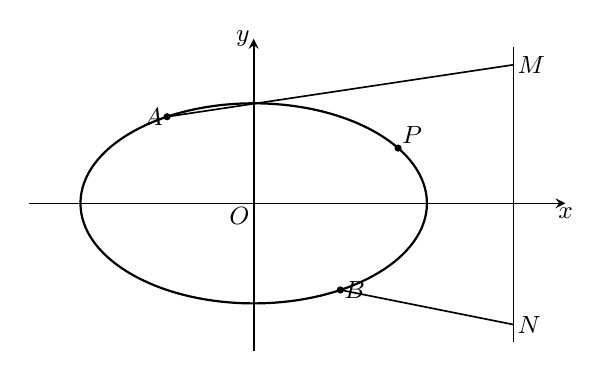
\begin{tikzpicture}[semithick, x=1.1cm, y=1.1cm, every node/.style={inner sep=1.2pt, font=\small}]
  \draw[-stealth] (-2.6,0) -- (3.6,0) node[below] {$x$};
  \draw[-stealth] (0,-1.7) -- (0,1.9) node[left] {$y$};
  \node[below left] at (0,0) {$O$};
  \draw[thick] (0,0) ellipse (2 and 1.155);
  \coordinate (A) at (-1,1);
  \coordinate (B) at (1,-1);
  \coordinate (P) at (1.667,0.638);
  \coordinate (M) at (3,1.6);
  \coordinate (N) at (3,-1.4);
  \fill (A) circle (1.3pt);
  \fill (B) circle (1.3pt);
  \fill (P) circle (1.3pt);
  \draw (A) -- (M);
  \draw (B) -- (N);
  \draw (3,-1.6) -- (3,1.8);
  \node[left] at (A) {$A$};
  \node[right] at (B) {$B$};
  \node[above right] at (P) {$P$};
  \node[right] at (M) {$M$};
  \node[right] at (N) {$N$};
\end{tikzpicture}
